\documentclass[conference]{IEEEtran}
\IEEEoverridecommandlockouts
% The preceding line is only needed to identify funding in the first footnote. If that is unneeded, please comment it out.
\usepackage{cite}
\usepackage{amsmath,amssymb,amsfonts}
\usepackage{algorithmic}
\usepackage{graphicx}
\usepackage{textcomp}
\usepackage{xcolor}
\usepackage[brazilian]{babel}
\usepackage[utf8]{inputenc}
\usepackage[T1]{fontenc}
\def\BibTeX{{\rm B\kern-.05em{\sc i\kern-.025em b}\kern-.08em
    T\kern-.1667em\lower.7ex\hbox{E}\kern-.125emX}}
\begin{document}

\title{Particle Swarm Optimization}

\author{Bruno Lopes}
\maketitle

\begin{abstract}
O objectivo deste artigo é conseguir implementar e avaliar a eficiência de Algoritmos de Otimização por Enxame de Partículas.

\end{abstract}

\section{INTRODUÇÃO}
	A otimização de enxame de partículas (PSO) é uma das técnicas evolutivas de computação. Como as outras técnicas de computação evolutiva, o PSO é um algoritmo de busca baseado na população e é inicializado com uma população de soluções aleatórias, chamadas partículas. Ao contrário das outras técnicas de computação evolucionária, cada partícula em PSO também está associada a uma velocidade. Partículas voam através do espaço de busca com velocidades que são ajustadas dinamicamente de acordo com seus comportamentos históricos. Portanto, as partículas tendem a voar em direção à melhor e melhor área de pesquisa ao longo do processo de busca. Desde sua introdução em 1995 \cite{b1}, a PSO atraiu muitas atenções de pesquisadores de todo o mundo. Muitos resultados de pesquisa foram relatados na literatura. Em 2003, o primeiro Simpósio IEEE sobre Inteligência de Enxame foi realizado em Indianápolis, Indiana, EUA. 
		
	As pesquisas sobre PSO geralmente podem ser categorizadas em cinco partes: algoritmos, topologia, parâmetros, algoritmos de PSO híbridos e aplicativos.

\section{Referencial Teórico}
	As idéias iniciais sobre os enxames de partículas de Kennedy (um psicólogo social) e Eberhart (um engenheiro elétrico) visavam essencialmente produzir inteligência computacional explorando análogos simples de interação social, em vez de habilidades cognitivas puramente individuais. As primeiras simulações \cite{b1} foram influenciadas pelo trabalho de Heppner e Grenander \cite{b2} e envolveram análogos de bandos de aves em busca de milho. Estes logo se desenvolveram (Kennedy e Eberhart, 1995; Eberhart e Kennedy, 1995; Eberhart et al., 1996) em um poderoso método de otimização - Optimização de Enxame de Partículas (PSO).

	No PSO, um número de entidades simples - as partículas - são colocadas no espaço de busca de algum problema ou função, e cada uma avalia a função objetivo em sua localização atual. Cada partícula determina seu movimento através do espaço de busca combinando algum aspecto da sua história de suas próprias localizações com as de um ou mais membros do enxame, com algumas perturbações aleatórias. A próxima iteração ocorre depois que todas as partículas foram movidas. 
	
	Eventualmente, o enxame como um todo, como um bando de pássaros em busca de comida coletivamente, provavelmente se aproxima de um ótimo da função de condicionamento físico.
	
	O enxame de partículas é mais do que apenas uma coleção de partículas. Uma partícula por si só quase não tem poder para resolver qualquer problema; o progresso ocorre apenas quando as partículas interagem.

	Cada partícula se comunica com algumas outras partes e é afetada pelo melhor ponto encontrado por qualquer membro de sua vizinhança topológica. 

	O algoritmo básico de otimização por enxame de partículas pode ser descrito brevemente utilizando os seguintes passos: dada uma população inicial de partículas, atualiza-se o vetor posição a partir do vetor velocidade de cada partícula até que se atinja o critério de parada pré-definido. 
	
	A figura abaixo ilustra essa lógica:
	
	\begin{figure}[htbp]
	\centerline{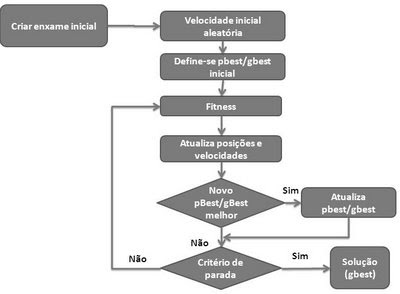
\includegraphics[scale=0.4]{pso_algoritmo.JPG}}
	\caption{Fluxograma-Algoritmo PSO}
	\label{fig}
	\end{figure}
	
	O enxame é inicializado com os valores dos vetores de velocidade e posição gerados aleatoriamente. A primeira iteração do algoritmo inicia com a atribuição de valores aos parâmetros da equação de velocidade. Definem-se então os valores referentes ao enxame, constantes e o critério de parada. Tendo já definido os valores para posição das partículas e suas respectivas velocidades, aplica-se o cálculo do fitness a cada partícula desta população. Conforme explicado anteriormente, o fitness avalia o desempenho da partícula. Com as partículas do enxame avaliadas, extraem-se os pbest e o gbest, isto é, a melhor posição encontrada pela partícula e pelo enxame. Depois as velocidades e as posições de cada partícula do enxame são atualizadas. Diante das novas posições, caso o critério de parada tenha sido atingido, a solução do problema encontrada é apresentada. Caso contrário, aplica-se novamente o fitness a este enxame, atualizam-se os valores de pbest e gbest, caso seja apresentada uma solução melhor, seguido da velocidade e posição de cada partícula do enxame. O laço prossegue até o critério de parada ter sido atingido.
    
    
\section{Metodologia Experimental}
    
    Em geral, um AG possui duas categorias de parâmetros da pesquisa experimental: qualitativos e quantitativos. Os principais parâmetros qualitativos são os tipos de crossover (um ponto, dois pontos e múltiplos pontos) e os métodos de seleção (proporcional, escalonamento, Boltzmann, ranque- amento e tournament). Os principais parâmetros quantitativos são constituídos pelo tamanho da população (n), pela taxa de crossover (TC) e pela taxa de mutação (Tm).
    
	\begin{figure}[htbp]
    \begin{center}
    	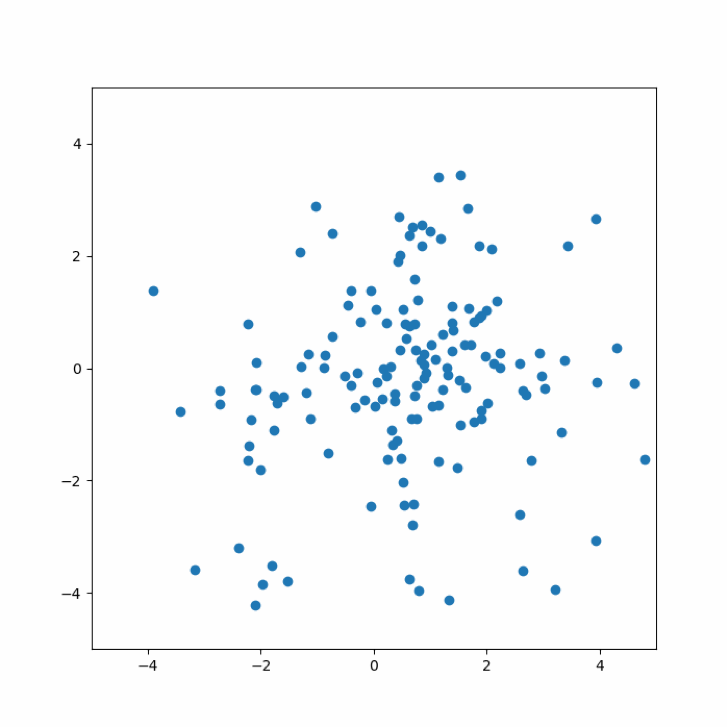
\includegraphics[scale=0.3]{imagens-pso/particle-swarm-optimization-01.png} 
        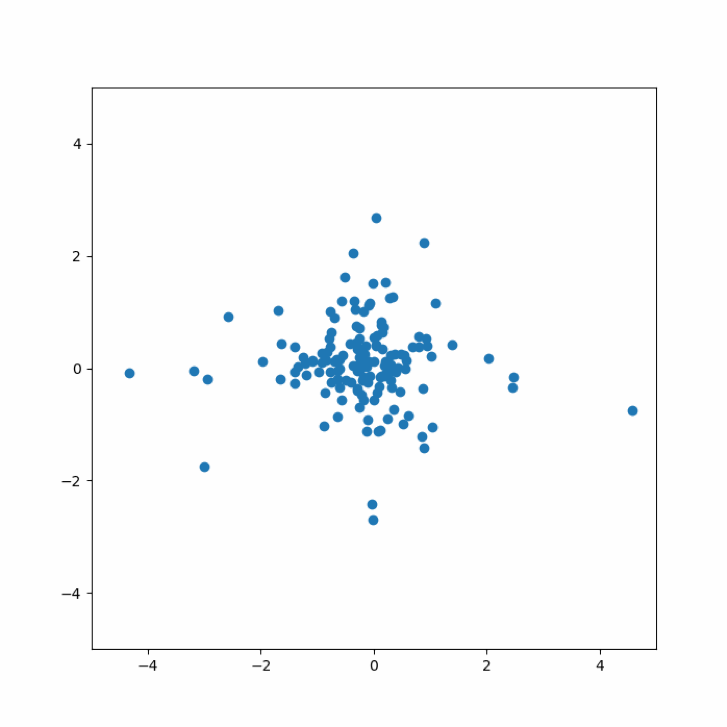
\includegraphics[scale=0.3]{imagens-pso/particle-swarm-optimization-02.png}
        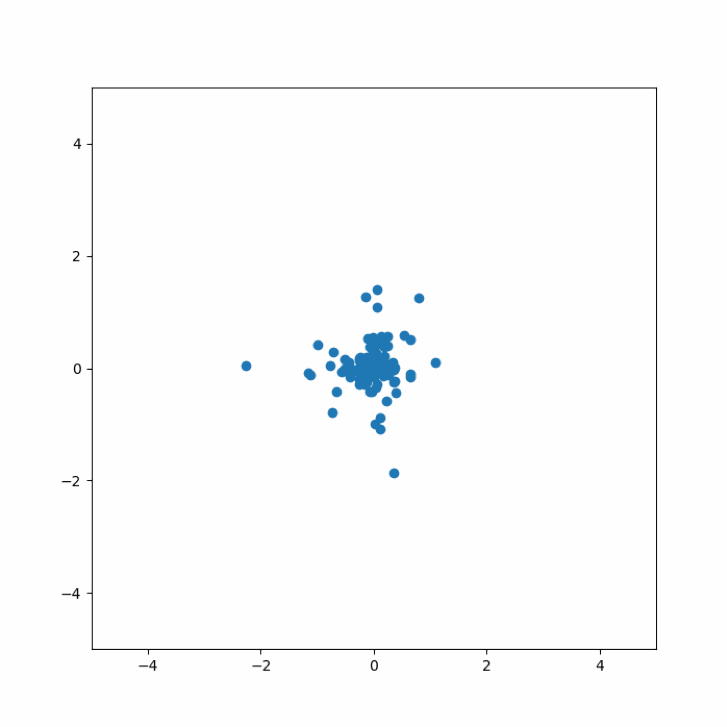
\includegraphics[scale=0.3]{imagens-pso/particle-swarm-optimization-03.png}
        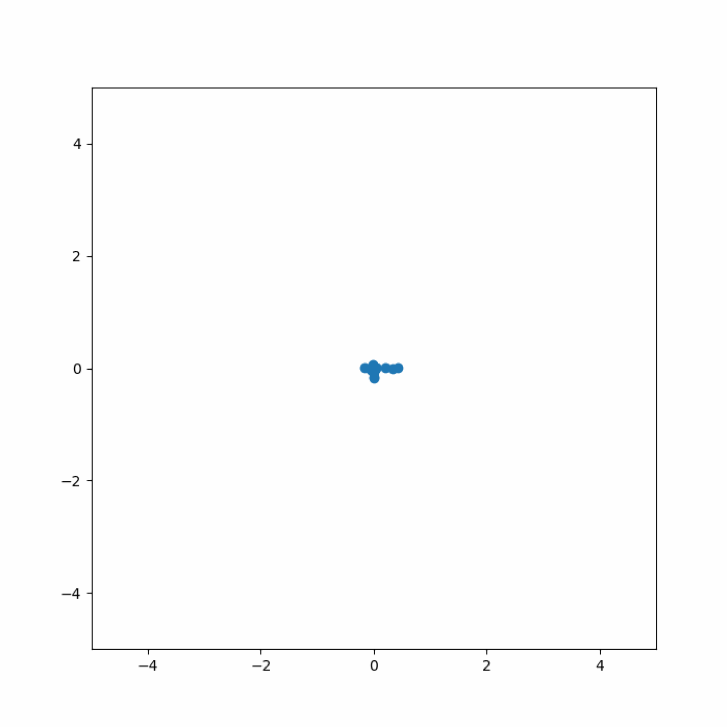
\includegraphics[scale=0.3]{imagens-pso/particle-swarm-optimization-04.png}
    \caption{Algoritmo padrão} \label{gdimotes}
    \end{center}
    \end{figure}

	\begin{figure}[htbp]
    \begin{center}
    	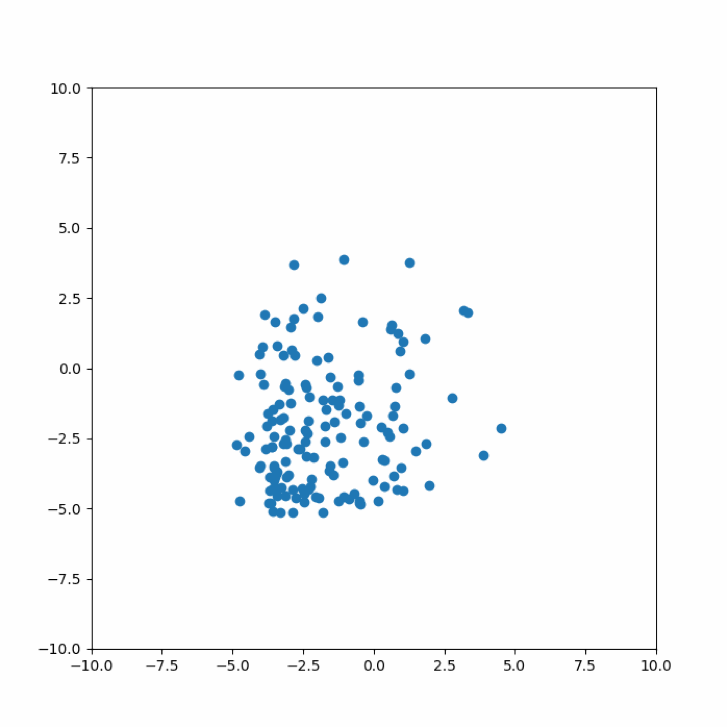
\includegraphics[scale=0.3]{imagens-pso/particle-swarm-optimization-leader-moving-01.png}
    	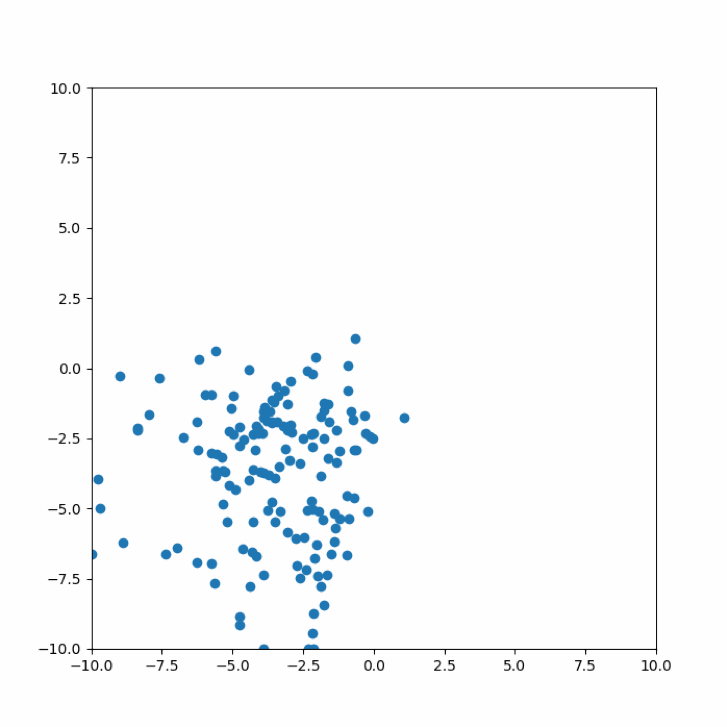
\includegraphics[scale=0.3]{imagens-pso/particle-swarm-optimization-leader-moving-02.png}
    	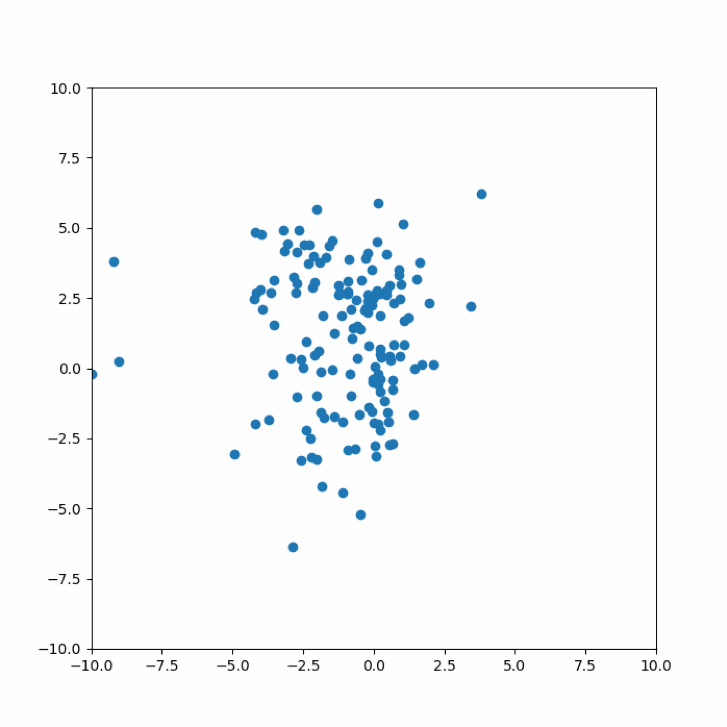
\includegraphics[scale=0.3]{imagens-pso/particle-swarm-optimization-leader-moving-03.png}
    	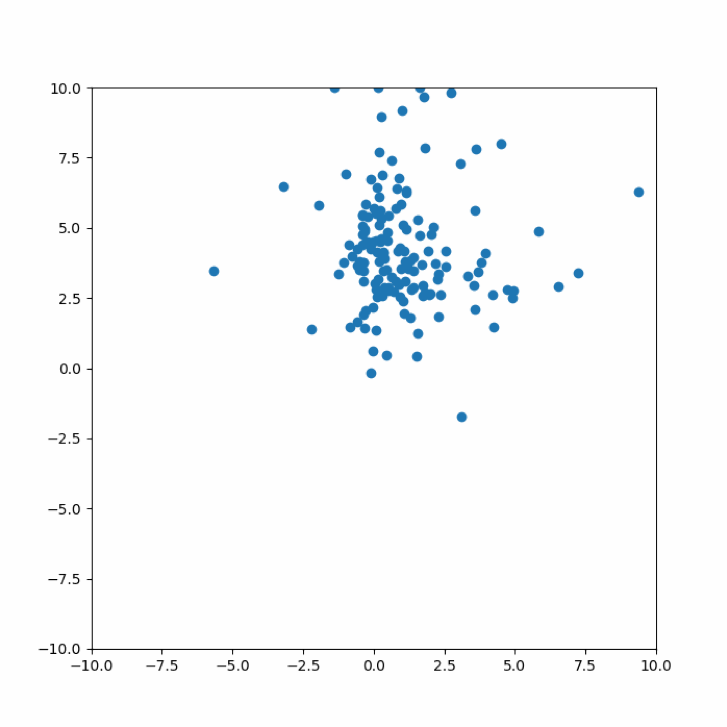
\includegraphics[scale=0.3]{imagens-pso/particle-swarm-optimization-leader-moving-04.png}    	
    \caption{Motes instalados na Great Duck Island} \label{gdimotes}
    \end{center}
    \end{figure}

\section{Resultado e Discussão}



\section*{Conclusão}




\begin{thebibliography}{00}

\bibitem{b1} Kennedy, J., and Eberhart, R. C.. (1995). Particle swarm optimization, Proc. of IEEE International Conference on Neural Networks (ICNN), Vol.IV, pp.1942-1948, Perth, Australia, 1995.
\bibitem{b2} Heppner, H., \& Grenander, U. (1990). A stochastic non-linear model for coordinated bird flocks. In S. Krasner
(Ed.), The ubiquity of chaos (pp. 233–238). Washington: AAAS.
\end{thebibliography}
\vspace{12pt}

\end{document}
